%%%%%%%%%%%%%%%%%%%%%%%%%%%%%%%%%%%%%%%%%%%%%%%%%%%
%
%  Main document template code for TAMU Theses and 
%  Dissertations starting Fall 2016.
%
%  Author:  Kyle R. Wodzicki  
%  Version: 0.17.09
%  Updated: 18 Jan. 2018
%
%  Adapted loosely from: 
%    TAMU LaTeX (SZR) Version 3.16.10 from OGAPS 
%
%%%%%%%%%%%%%%%%%%%%%%%%%%%%%%%%%%%%%%%%%%%%%%%%%%%
% To change left margin for binding purposes
%    [12pt,binding]
% To change document spacing to 1.5 spacing
%    [12pt,onehalfspacing]
% To place a 'Reference' section at the end
% of each chapter, use the 'chapref' option
%    [12pt,chapref]
% Can combine options
\documentclass[12pt]{tamu_thesis}   	% Load the tamu_thesis document class

%%%%%%%%%%%%%%%%%%%%%%%%%%%%%%%%%%%%%%%%%%%%%%%%%%%%
%%%          Load extra packages here            %%%
%%%%%%%%%%%%%%%%%%%%%%%%%%%%%%%%%%%%%%%%%%%%%%%%%%%%
\usepackage[colorlinks=false]{hyperref}	% hyperref with coloring and footnote do NOT get along
\usepackage{multirow}			% Multirow package for tables
\usepackage{footnote}			% Package for the savenotes command
\usepackage{amsthm}				% AMS package for theorems
%\usepackage{natbib,url}			% Load the natbib and ulr packages

%%%%%%%%%%%%%%%%%%%%%%%%%%%%%%%%%%%%%%%%%%%%%%%%%%%%
%%%       Set information for title page.        %%%
%%%%%%%%%%%%%%%%%%%%%%%%%%%%%%%%%%%%%%%%%%%%%%%%%%%%
% Delete or comment out tags that are NOT needed
\Title{The Title of Your Thesis or Dissertation Goes In This Space To Let Us Know What Your Document is About}
\PaperType{Thesis}					% Enter the paper type
\FullName{Aggie D. Student}			% Enter full name
\Degree{Master of Science}			% Enter degree
\Chair{Chair Name}					% Enter name of committee chair
%\CoChair{Co-Chair Name}			% Enter name of committee co-chair
\MemberOne{Committee Member 1}		% Name of first committee member
\MemberTwo{Committee Member 2}		% Name of second committee member
\MemberThree{Committee Member 3}	% Name of third committee member
%\MemberFour{Committee Member 4}	% Name of fourth committee member
\DeptHead{Head of Department}		% Enter name of department head
\GradMonth{December}				% Enter graduation month
\GradYear{2016}						% Enter graduation year
\Dept{Mathematics}					% Enter department name	

\bibfile{myReference}               % Set the bibliography file to use
\bibstyle{ieeetr}                   % Set the bibliography style to use
%%%%%%%%%%%%%%%%%%%%%%%%%%%%%%%%%%%%%%%%%%%%%%%%%%%%%%
%%%  Set path to the figures and figure extensions %%%
%%%%%%%%%%%%%%%%%%%%%%%%%%%%%%%%%%%%%%%%%%%%%%%%%%%%%%
\graphicspath{ {./graphic/},{./figures/}  } % Locations of figures
\DeclareGraphicsExtensions{.png,.PNG,.jpg}  % Figure extensions

%%%%%%%%%%%%%%%%%%%%%%%%%%%%%%%%%%%%%%%%%%%%%%%%%%%%%%
% Define custom  commands for easier typing        %%%
%%%%%%%%%%%%%%%%%%%%%%%%%%%%%%%%%%%%%%%%%%%%%%%%%%%%%%
\newcommand{\mmday}{mm day$^{-1}$}  % Command for mm day^-1 units

%%%%%%%%%%%%%%%%%%%%%%%%%%%%%%%%%%%%%%%%%%%%%%%%%%%%
%%% Load the nomenclature package. Default is to  
%%% display all the nomenclature/acronyms. Remove
%%% the [all] option to display only those used.
\usepackage[all]{nomenclature}

%%%%%%%%%%%%%%%%%%%%%%%%%%%%%%%%%%%%%%%%%%%%%%%%%%%%
%%%          Beginning of the document           %%%
%%%%%%%%%%%%%%%%%%%%%%%%%%%%%%%%%%%%%%%%%%%%%%%%%%%%
\begin{document}
\maketitle			% Must have this to generate the title page!!!

% Be sure to include all TeX files to be used in your document!
% !TEX root = ../TAMU_Thesis_Main.tex

%%%%%%%%%%%%%%%%%%%%%%%%%%%%%%%%%%%%%%%%%%%%%%%%%%%%%%%%%%%%%%%%%%%%%
%%                           ABSTRACT 
%%%%%%%%%%%%%%%%%%%%%%%%%%%%%%%%%%%%%%%%%%%%%%%%%%%%%%%%%%%%%%%%%%%%%

\begin{abstract}

This is the first numbered page, lower case Roman numberal (ii). Page numbers are outside the prescribed margins, at the bottom of the page and centered; everything else is inside the margins.No bold on this page (Exception: heading ABSTRACT is bold if major headings are bold. \emph{This \LaTeX ~ template applies to this exception}).

Text begins two double spaces below the major heading. Recommended length of text is no more than 350 words. Vertical spacing is double spaced or space-and-a-half. (\emph{This \LaTeX ~ template applies double space for this ABSTRACT.}) The same margin settings and text alignment are followed else where in this thesis. There should be no numbered references or formal citations in ABSTRACT.

The content of this ABSTRACT provides a complete, succinct snapshot of the research, addressing the purpose, methods, results, and conclusions of the research. As a result, it should stand alone without any formal citations or references to chapters/sections of the work. To accomodate with a variety of online database, images or complex equations should also be avoided.

The next pages are Dedication, Acknowledgments, Contributors and Funding Sources, and Nomenclature. Of these, Contributors and Funding Sources is required. The rest are optional.

\end{abstract}			% Include the abstract.tex file
%%%%%%%%%%%%%%%%%%%%%%%%%%%%%%%%%%%%%%%%%%%%%%%%%%%
%
%  New template code for TAMU Theses and Dissertations starting Fall 2016.  
%
%  Author: Sean Zachary Roberson
%	 Version 3.16.09
%  Last updated 9/12/2016
%
%  Modified 04 Nov. 2016 by Kyle R. Wodzicki
%%%%%%%%%%%%%%%%%%%%%%%%%%%%%%%%%%%%%%%%%%%%%%%%%%%

%%%%%%%%%%%%%%%%%%%%%%%%%%%%%%%%%%%%%%%%%%%%%%%%%%%%%%%%%%%%%%%%%%%%%%
%%                           DEDICATION
%%%%%%%%%%%%%%%%%%%%%%%%%%%%%%%%%%%%%%%%%%%%%%%%%%%%%%%%%%%%%%%%%%%%%
\begin{dedication}


\begin{center}
\vspace*{\fill}
To my mother, my father, my grandfather, and my grandmother. To see what happens with multiple lines, I extend this next part into a second line.
\vspace*{\fill}
\end{center}

\end{dedication}			% Include the dedication file
% !TEX root = ../TAMU_Thesis_Main.tex

%%%%%%%%%%%%%%%%%%%%%%%%%%%%%%%%%%%%%%%%%%%%%%%%%%%%%%%%%%%%%%%%%%%%%%
%%                           ACKNOWLEDGMENTS
%%%%%%%%%%%%%%%%%%%%%%%%%%%%%%%%%%%%%%%%%%%%%%%%%%%%%%%%%%%%%%%%%%%%%
\begin{acknowledgements}

This section is also optional, limited to four pages. It must follow the Dedication Page (or Abstract, if no Dedication). If listing preliminary pages in Table of Contents, include Acknowledgments. Heading (\MakeUppercase{Acknowledgments}) is bold if major headings are bold. It should be in same type size and style as text. So does vertical spacing, paragraph style, and margins. Also, ensure that the spelling of ``acknowledgments'' matches throughout the text and the table of contents.

I would like to thank the Texas A\&M University Office of Graduate and Professional Studies to allow me to construct this \LaTeX\ thesis template. Special thanks to JaeCee Crawford, Amy Motquin, Ashley Schmitt, Rachel Krolczyk, and Roberta Caton for carefully reviewing this material.  % use A\&M instead of A$\&$M, not use $A\&M$ as well, the last one won't be bold.


\end{acknowledgements}	% Include the acknowledgements file
% !TEX root = ../TAMU_Thesis_Main.tex

%%%%%%%%%%%%%%%%%%%%%%%%%%%%%%%%%%%%%%%%%%%%%%%%%%%%%%%%%%%%%%%%%%%%%%
%%             CONTRIBUTORS AND FUNDING SOURCES
%%%%%%%%%%%%%%%%%%%%%%%%%%%%%%%%%%%%%%%%%%%%%%%%%%%%%%%%%%%%%%%%%%%%%

\begin{contributors}

%This section is taken directly from the MS Word templates.

%Old version below.

%All theses and dissertations must include a contributors and funding sources section. In this section, name all members of the dissertation committee, and any collaboration with others in carrying out your thesis or dissertation research. Your independent contributions must be made clear.
%
%If financial support from the university or any other source was gained to conduct your thesis or dissertation research and compilation, it must be listed in this section. If you completed all work independently without outside financial support, indicate this here.
%\textit{(Sample Wording)}
%
%This work was supported by a dissertation committee consisting of Professor XXX [advisor – also note if co-advisor] and XXXX of the Department of [Home Department] and Professor(s) XXXX of the Department of [Outside Department].
% 
%The data analyzed for Chapter III was provided by Professor XXXX. The analyses depicted in Chapter IV were conducted in part by Rebecca Jones of the Department of Biostatistics and were published in (year) in an article listed in the Biographical Sketch. 
%
%All other work conducted for the dissertation was completed by the student independently.
%
%\noindent \textit{(or)}
%
%This work was supervised by a dissertation committee consisting of Professor XXXX [advisor – also note if co-advisor] and Professor(s) XXXX of the Department of [Home Department] and Professor(s) XXXX of [Outside Department]. All work for the dissertation was completed independently by the student.
%
%\noindent \textit{(or)}
%
%Graduate study was supported by a fellowship from Texas A\&M University and a dissertation research fellowship from XXX Foundation.

\subsection*{Contributors}
This work was supported by a thesis (or) dissertation committee consisting of Professor XXXX [advisor --– also note if co-advisor] and XXX of the Department of [Home Department] and Professor(s) XXXX of the Department of [Outside Department].

The data analyzed for Chapter X was provided by Professor XXXX. The analyses depicted in Chapter X were conducted in part by Rebecca Jones of the Department of Biostatistics and were published in (year) in an article listed in the Biographical Sketch.

All other work conducted for the thesis (or) dissertation was completed by the student independently.
\subsection*{Funding Sources}
Graduate study was supported by a fellowship from Texas A\&M University and a dissertation research fellowship from XXX Foundation. 

\end{contributors}		% Include the contributors file
\makeNomenclature					% Generate nomenclature if using the nomenclature package

\makeToC							% Generate the Table of Contents. REQUIRED!!!

% Include all chapters of the 
% thesis. Note that you MUST  
% use the \chapInclude command
\chapInclude{./Data/Section1}		% Include the Section1.tex file
\chapInclude{./Data/Section2}		% Include the Section2.tex file
\chapInclude{./Data/Section3}		% Include the Section3.tex file
\chapInclude{./Data/Section4}		% Include the Section4.tex file

%%%%%%%%%%%%%%%%%%%%%%%%%%%%%%%%%%%%%%%%%%%%%%%%%%%%
% Generate the Bibliography DO NOT TOUCH THIS!!!
\ifchapref\else\makebibliography\fi

%%%%%%%%%%%%%%%%%%%%%%%%%%%%%%%%%%%%%%%%%%%%%%%%%%%%
% Include appendices. 
% MUST BE IN APPENDICES ENVIRONMENT!!!
\begin{appendices}
	% !TEX root = ../TAMU_Thesis_Main.tex
%%%%%%%%%%%%%%%%%%%%%%%%%%%%%%%%%%%%%%%%%%%%%%%%%%%
%
%  New template code for TAMU Theses and Dissertations starting Fall 2016.
%
%
%  Author: Sean Zachary Roberson 
%	 Version 3.16.09
%  Last updated 9/12/2016
%
%  Modified 04 Nov. 2016 by Kyle R. Wodzicki
%%%%%%%%%%%%%%%%%%%%%%%%%%%%%%%%%%%%%%%%%%%%%%%%%%%

%%%%%%%%%%%%%%%%%%%%%%%%%%%%%%%%%%%%%%%%%%%%%%%%%%%%%%%%%%%%%%%%%%%%%%
%%                           APPENDIX A 
%%%%%%%%%%%%%%%%%%%%%%%%%%%%%%%%%%%%%%%%%%%%%%%%%%%%%%%%%%%%%%%%%%%%%

%\phantomsection

\chapter{First Appendix}\label{appendix:01}

Text for the Appendix follows.

\begin{figure}[h]
\centering
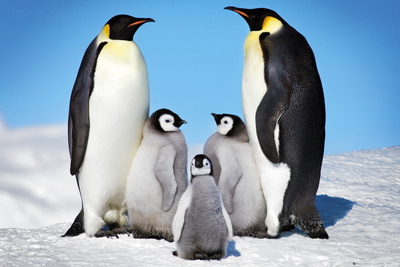
\includegraphics[scale=.50]{figures/Penguins.jpg}
\caption{TAMU figure}
\label{fig:tamu-fig5}
\end{figure}
			% Include the appendix1.tex file
	%%%%%%%%%%%%%%%%%%%%%%%%%%%%%%%%%%%%%%%%%%%%%%%%%%%
%
%  New template code for TAMU Theses and Dissertations starting Fall 2012.  
%  For more info about this template or the 
%  TAMU LaTeX User's Group, see http://www.howdy.me/.
%
%  Author: Wendy Lynn Turner 
%	 Version 1.0 
%  Last updated 8/5/2012
%
%%%%%%%%%%%%%%%%%%%%%%%%%%%%%%%%%%%%%%%%%%%%%%%%%%%

%%%%%%%%%%%%%%%%%%%%%%%%%%%%%%%%%%%%%%%%%%%%%%%%%%%%%%%%%%%%%%%%%%%%%%
%%                           APPENDIX B
%%%%%%%%%%%%%%%%%%%%%%%%%%%%%%%%%%%%%%%%%%%%%%%%%%%%%%%%%%%%%%%%%%%%%

\chapter{\uppercase {Second Appendix with a longer title - much longer in fact}}

Text for the Appendix follows.

\begin{figure}[H]
\centering
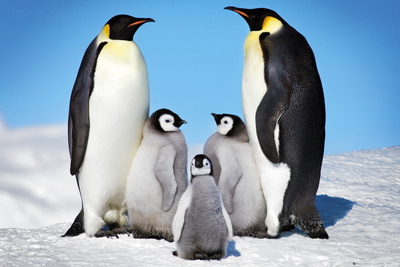
\includegraphics[scale=.50]{figures/Penguins.jpg}
\caption{TAMU figure}
\label{fig:tamu-fig6}
\end{figure}

\section{Appendix Section}


\pagebreak{}			% Include the appendix2.tex file
	% !TEX root = ../TAMU_Thesis_Main.tex
%%%%%%%%%%%%%%%%%%%%%%%%%%%%%%%%%%%%%%%%%%%%%%%%%%%
%
%  New template code for TAMU Theses and Dissertations starting Fall 2016.
%
%
%  Author: Sean Zachary Roberson 
%	 Version 3.16.09 
%  Last updated 9/12/2016
%
%  Modified 04 Nov. 2016 by Kyle R. Wodzicki
%%%%%%%%%%%%%%%%%%%%%%%%%%%%%%%%%%%%%%%%%%%%%%%%%%%

%%%%%%%%%%%%%%%%%%%%%%%%%%%%%%%%%%%%%%%%%%%%%%%%%%%%%%%%%%%%%%%%%%%%%%
%%                           APPENDIX B
%%%%%%%%%%%%%%%%%%%%%%%%%%%%%%%%%%%%%%%%%%%%%%%%%%%%%%%%%%%%%%%%%%%%%

\chapter{Bibliography Information}\label{appendix:02}

As previously mentioned, one program that can be used to organize references is \href{http://www.jabref.org}{\textbf{JabRef}}. While a tutorial of how to use \textbf{JabRef} is beyond the scope of this template, a brief discussion of how to use \textbf{BibTeX} follows.

\section{BibTeX}
After you have installed \textbf{JabRef}, or any citation manager of your choosing that is compatible with \textbf{BibTeX}, you must create a \textbf{BibTeX} database. This database file will contain all the information \textbf{BibTeX} requires to generate your bibliography. An example .bib file named `myReference.bib' is included in this template. The first entry of that file is shown below.

{\footnotesize \begin{verbatim}
@Article{Barn-JORVQ,
  author  = {Christopher F. Barnes and Richard L. Frost},
  title   = {Residual Vector Quantizers with Jointly Optimized Code Books},
  journal = {Advances in Electronics and Electron Physics},
  year    = {1992},
  volume  = {84},
  pages   = {1--59},
}
\end{verbatim}}

All of the entries in the entry are very self-explanatory, such as author and title, however, arguably the most important part of the entry is the key. The key is the first value after @Article, which is Barn-JORVQ in this example. This is the key you will use in any cite commands for references, e.g.,

{\footnotesize\begin{verbatim}\cite{Barn-JORVQ}\end{verbatim}}.


Depending on the citation style that is used, there may be different cite commands for different types of in-text citations. It is important to know which commands must be used with the citation style you are using.

\section{Compiling with BibTeX}
When compiling your \LaTeX{} document, it is also important to remember to compile it twice to ensure that all equation, fig, table, etc. cross-references have updated correctly. However, when using citations from a .bib file in your document, the process is a little longer. To ensure that your bibliography generates correctly, one must run XeLaTeX, then BibTeX, then XeLaTeX twice. This will ensure that all the citations and cross-references are updated correctly. If you are using a program such as \textbf{MikTeX} or \textbf{ProTeXt}, this may be the default compilation method. However, if you use \textbf{TeXShop} on a Mac, you must change the compiler manually. If compiling from command line, the sequence would be:

{\footnotesize \begin{verbatim}
xelatex TAMU_Thesis_Main.tex
bibtex TAMU_Thesis_Main.aux
xelatex TAMU_Thesis_Main.tex
xelatex TAMU_Thesis_Main.tex
\end{verbatim}}

Be sure to check the output for any errors. If question marks (?) appear in any location where a reference should be, there was an issue with the compilation. Make certain that the key used in the cite command matches the corresponding references in the .bib file.

\section{References at the end of chapters}
If you would like references at the end of each chapter, first make sure you are using the `chapref' options in the documentclass command at the top of the Main \LaTeX document. Once that option is set, compilation is similar to the method discussed above.

First, compile the main file use XeLaTeX. When it is done compiling, check the directory your document is saved in. There should be a bunch of files named `bu*.aux', where the asterisk represents any number. You will now want to run bibtex on all of these .aux files as well as the .aux file from the main document. After bibtex is run on all the .aux files, run XeLaTeX two more times and your document should be good to go! If you are on a Mac, open up a Terminal window, cd into the directory your document is in and run the following commands (should work on any Linux machine as well):

{\footnotesize \begin{verbatim}
xelatex TAMU_Thesis_Main.tex
find ./ -name '*.aux' -exec bibtex '{}' \;
xelatex TAMU_Thesis_Main.tex
xelatex TAMU_Thesis_Main.tex
\end{verbatim}}
The second command simply finds all the .aux files in the current working directory and executes (exec) the command bibtex on each of them.

Be sure to check the output for any errors. If question marks (?) appear in any location where a reference should be, there was an issue with the compilation. Make certain that the key used in the cite command matches the corresponding references in the .bib file.			% Include the appendix3.tex file
\end{appendices}

\end{document}